\section{Methodology}
\label{sec:Methodology}

The goal of this project is to create VeriTest: an Automated Testing Framework for GraalVM's optimization DSL. This will represent another 
tool that the developers of GraalVM could use to provide a \emph{certificate} for their implementation code. To assist in verifying the 
optimization rule, the tool would need to be able to classify each of the optimization rules (See Fig. \ref{fig:classification}). Furthermore, 
there are several key non-functional requirements for the system that need to be satisfied (See Fig. \ref{fig:requirements}).

\begin{figure}[h]
      \begin{tabular}{|L{0.95\textwidth}|}
            \hline
            \begin{enumerate}
                  \item The optimization rule is obviously false;
                  
                        This would require the tool to generate obvious counterexamples via Quickcheck (See \ref{sec:Quickcheck}) or Nitpick 
                        (See \ref{sec:Nitpick}).
              
                  \item The optimization rule is obviously true;
                  
                        This would require the tool to verify that Sledgehammer (See \ref{sec:Quickcheck}) can provide proof obligations for the 
                        optimization rule \textbf{without} dynamically defining proof tactics.
              
                  \item The optimization rule would require manual proving by \emph{"proof experts"}.
                        
                        This means that the optimization is non-trivial: Isabelle is not able to find an obvious counterexample, and proving would require 
                        additional tactics or sub-goals to be defined.
            \end{enumerate} \\
            \hline
      \end{tabular}
      \caption{The classification of an optimization rule}
      \label{fig:classification}
\end{figure}

\begin{figure}[h]
      \begin{tabular}{|L{0.95\textwidth}|}
            \hline
            \begin{enumerate}
                  \item Developers of GraalVM need to be able to integrate this easily into their test suite;
                  \item Developers of GraalVM can easily use this without understanding Isabelle;
                  \item \emph{If possible}, the system doesn't require enormous computing resources locally.
            \end{enumerate} \\
            \hline
      \end{tabular}
      \caption{Non-functional requirements of the Framework}
      \label{fig:requirements}
\end{figure}

To implement the tool, it would require the project to explore whether it is even possible to utilize Isabelle as the core system of the framework. 
Hence, understanding Isabelle's implementation is crucial to realize the goals of this project. At a glance, there are three options 
to the project:

\begin{itemize}
    \item Utilize Isabelle Client - Server interactions (See Sec. \ref{sec:IsabelleServer});
    \item Extend Isabelle/Scala (See Sec. \ref{sec:IsabelleScala});
    \item Utilize Isabelle CLI (See Sec. \ref{sec:IsabelleCLI})
    \item Create an Interpreter for GraalVM's optimization DSL (See Sec. \ref{sec:DSLInterpreter}).
\end{itemize}

\begin{figure}[h]
      \centering
      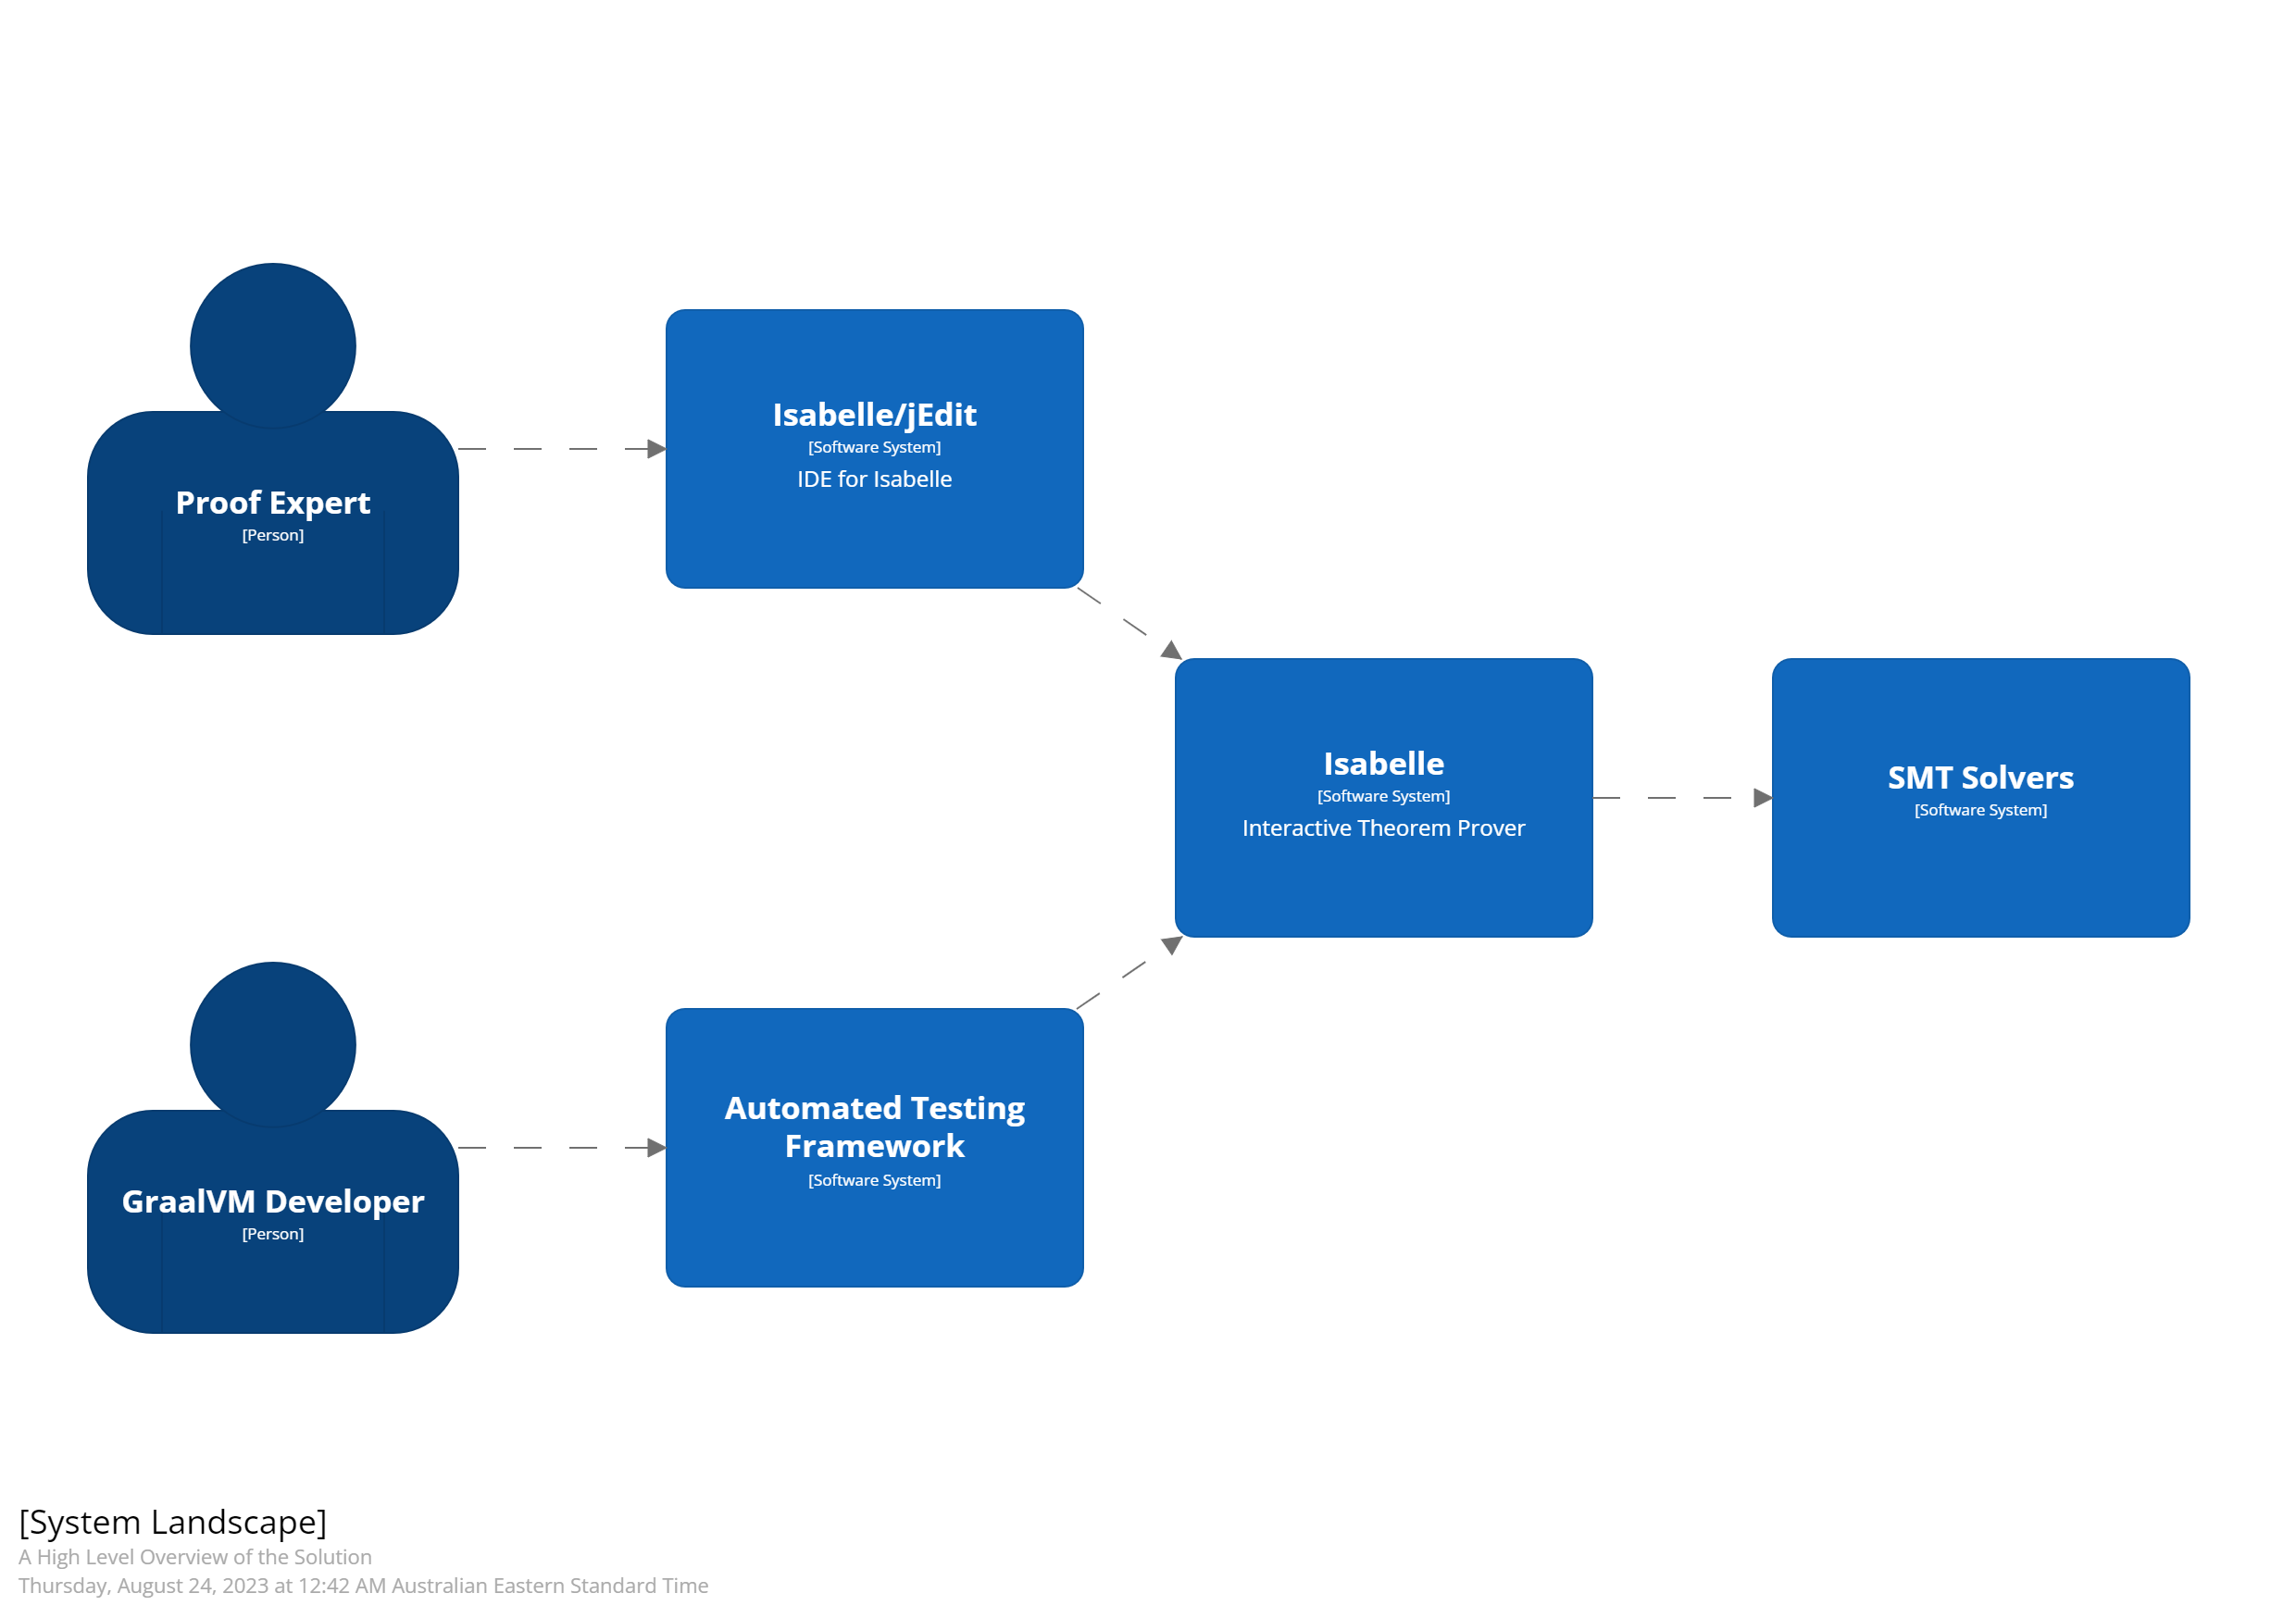
\includegraphics[width=1\textwidth]{structurizr-1-framework_overview_1.png}
      \caption{Proposed Solution}
      \label{fig:SystemLandscape}
\end{figure}

Fig. \ref{fig:SystemLandscape} depicts the overview of the proposed solution's system landscape. In theory, it would utilize Isabelle in a similar 
manner as Isabelle/jEdit \cite{isabelleSystem}. Therefore, it should be able to use the same Isabelle functionalities as Isabelle/jEdit does.

\subsection{Isabelle System Overview}
\label{sec:IsabelleSystemOverview}

\begin{figure}[h]
      \centering
      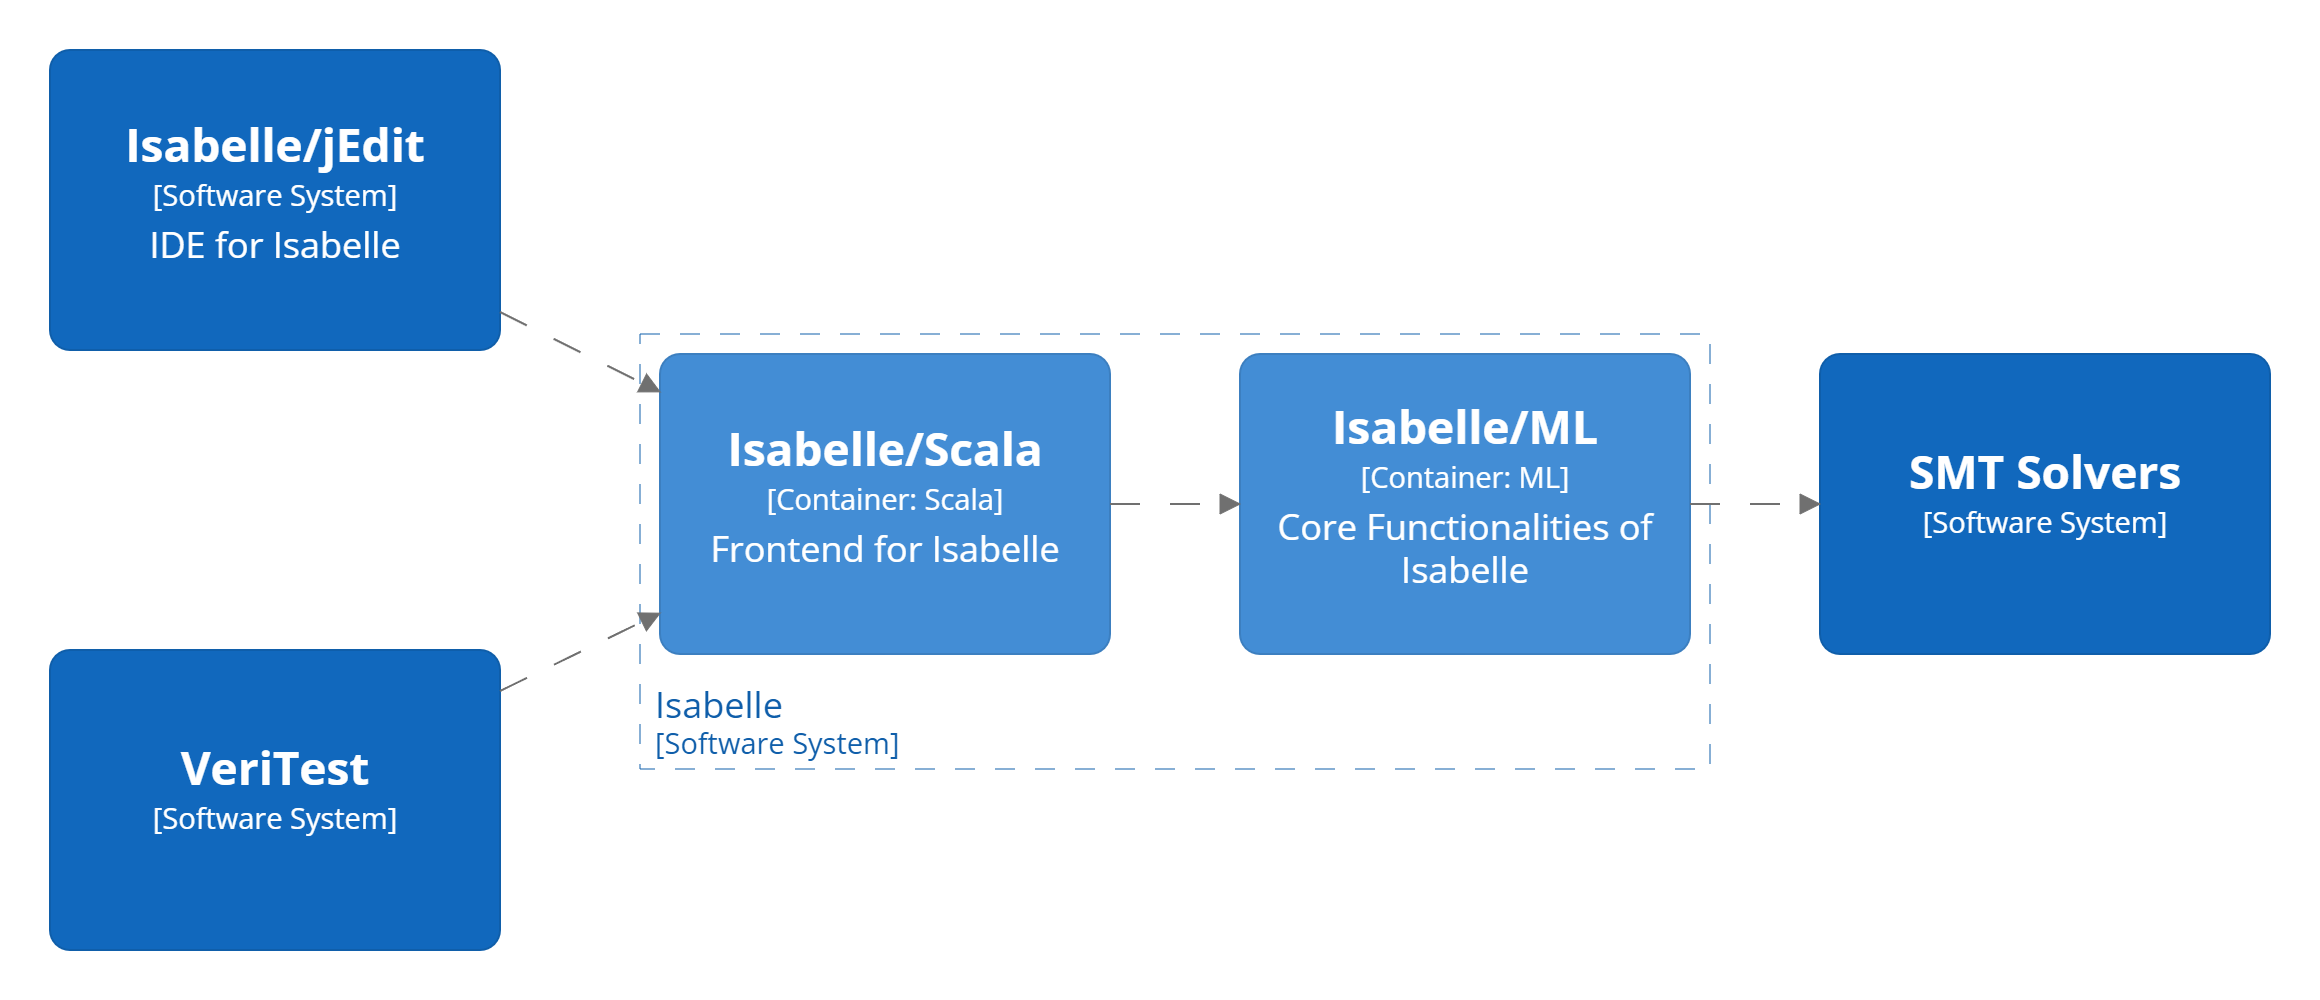
\includegraphics[width=1\textwidth]{structurizr-1-isabelle_overview_1.png}
      \caption{Isabelle System Overview}
      \label{fig:IsabelleSystem}
\end{figure}

Isabelle is made up of two significant components: Isabelle/ML and Isabelle/Scala \cite[Ch. 5]{isabelleSystem}. Isabelle/ML acts as the core 
functionality of Isabelle, harboring all the tools needed for proving theorems. Isabelle/Scala acts as the system infrastructure for Isabelle/ML 
-- hiding all the implementation details of Isabelle/ML.

\subsection{Utilizing Isabelle Server}
\label{sec:IsabelleServer}

\begin{figure}[h]
      \centering
      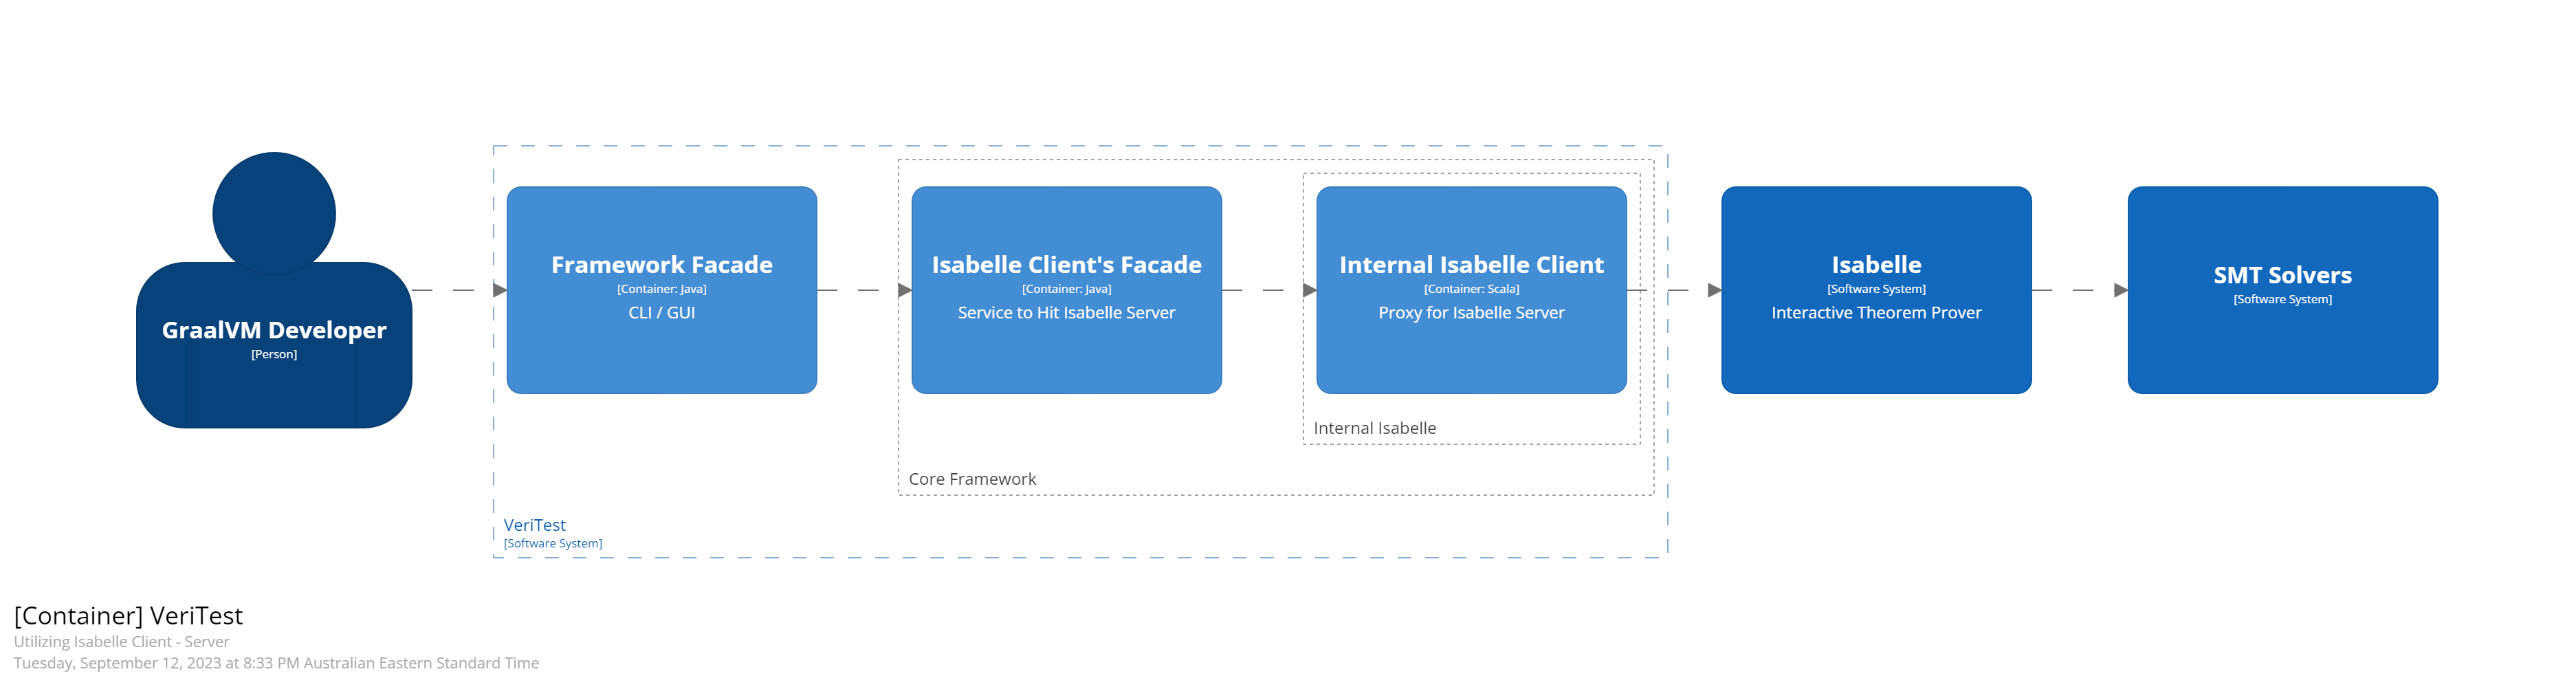
\includegraphics[width=1\textwidth]{structurizr-1-isabelle_client_server_1.png}
      \caption{Utilizing Isabelle Client - Server interaction}
      \label{fig:IsabelleServer}
\end{figure}

Isabelle Server acts as the core Isabelle process that allows theorems and all the required facts to be loaded up and processed by Isabelle/ML
\cite[Ch. 4]{isabelleSystem}. Interactions to Isabelle/Server would require a duplex socket connection over TCP \cite[Ch. 4.2]{isabelleSystem}. 
To simplify the communication between the framework and Isabelle/Server, we utilize Isabelle Client \cite[Ch. 4.1.2]{isabelleSystem} -- a proxy 
for Isabelle/Server that handles all the communication protocols of Isabelle/Server.

Isabelle Server can load theorems and process requests in parallel \cite[Ch. 4.2.6]{isabelleSystem}. As such, this solution would be ideal 
for the project, as it would allow the framework to offload the computing resources of loading and processing optimization proofs at external sites.
However, it would require a \emph{Facade} that implements a demultiplexer for asynchronous messages on Isabelle Client (See Fig. \ref{fig:IsabelleServer}). 
Furthermore, the full capabilities of Isabelle Server need to be explored to implement this option.

\subsection{Extending Isabelle/Scala}
\label{sec:IsabelleScala}

\begin{figure}[h]
      \centering
      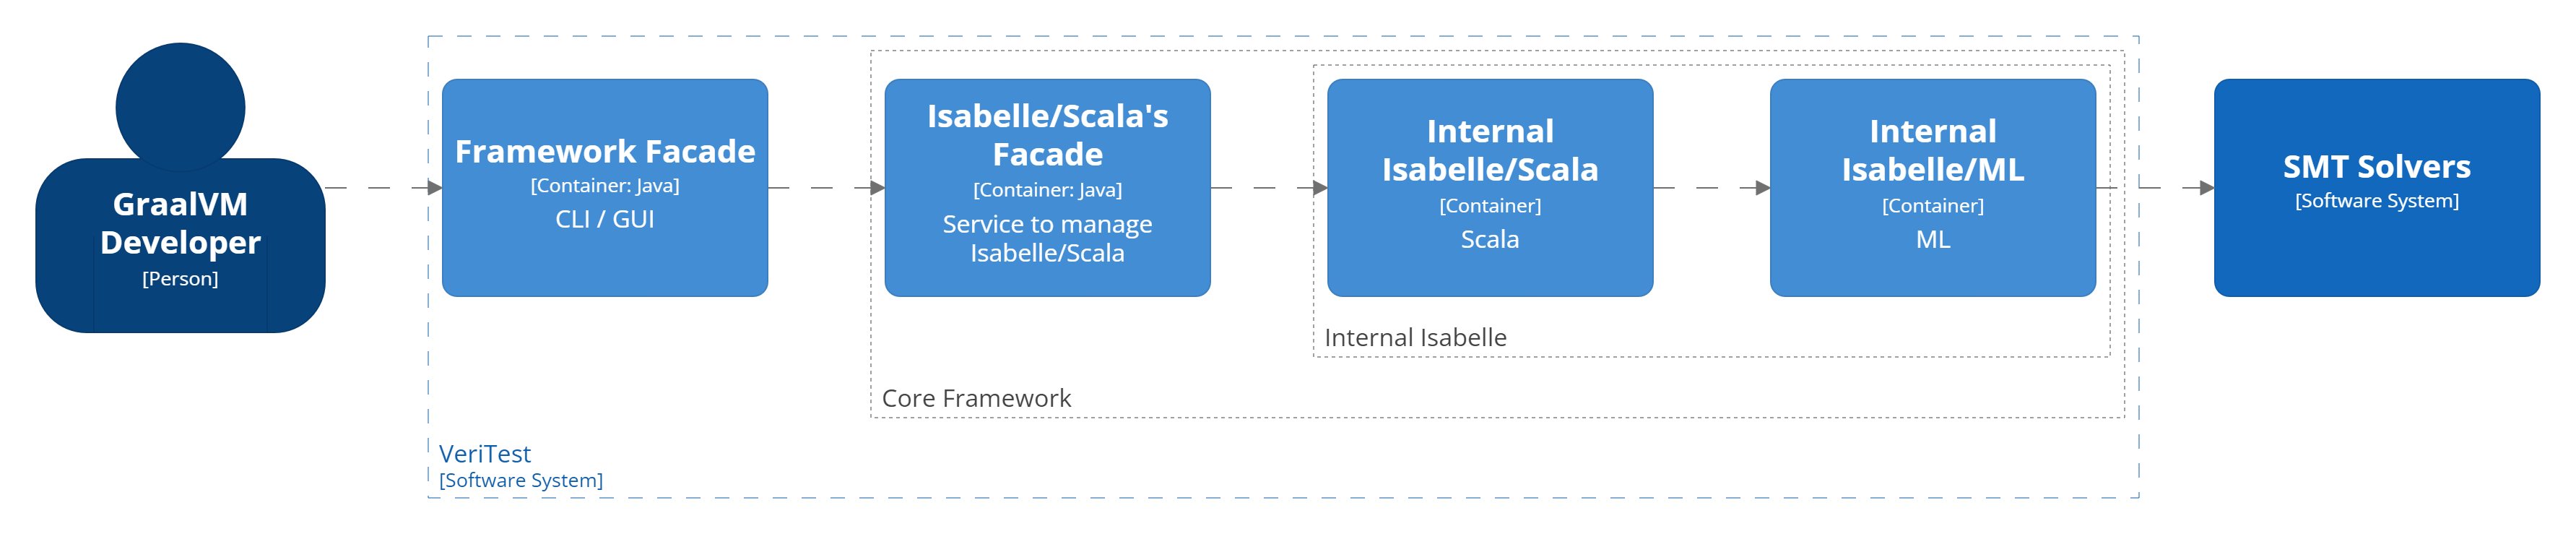
\includegraphics[width=1\textwidth]{structurizr-1-isabelle_scala_1.png}
      \caption{Extending Isabelle/Scala}
      \label{fig:IsabelleScala}
\end{figure}

Isabelle can be extended by accessing Isabelle/Scala functions \cite[Ch. 5]{isabelleSystem}. Extending Isabelle/Scala would require the framework 
to utilize Isablle's Scala compiler \cite[Ch. 5.1.4]{isabelleSystem}. Consequently, it means that Isabelle/ML would be bundled with Isabelle/Scala. 
As such, this option would be able to utilize all the functionalities of Isabelle. Fig. \ref{fig:IsabelleScala} depicts the proposed solution for 
this option.

However, the full complexity of Isabelle/Scala is unknown. Currently, Isabelle/Scala is not well documented and would require much of the 
project's timeline to understand Isabelle/Scala. Furthermore, extending Isabelle/Scala \emph{could} mean that the framework would take up 
much of the computing resources to execute Isabelle/ML functions locally.

\subsection{Utilizing Isabelle CLI}
\label{sec:IsabelleCLI}

Veriopt's current semi-automated approach \cite[Sec. 5.1]{Term_Graph_Optimizations} utilizes Isabelle CLI, a wrapper for Isabelle/Scala functions 
\cite{IsabelleHOL}. As such, this solution would represent an Isabelle management service, where each optimization rule will be passed into an 
Isabelle/Scala function inside an Isabelle process and managed accordingly. In essence, the solution is similar to Sec. \ref{sec:IsabelleScala}. 
However, the solution will require additional processing overhead in the form of multiple local Isabelle processes for each of the optimization rules, 
instead of a single VeriTest and Isabelle instance.

\subsection{Interpreter for DSL}
\label{sec:DSLInterpreter}

Building an interpreter for GraalVM's optimization DSL acts as a last resort to the project. To implement this, it would require a significant 
amount of time to rework the DSL into the framework, and designing tools similar to Quickcheck (See Sec. \ref{sec:Quickcheck}) in order to satisfy the 
system requirements. Reinventing the wheel would not be productive for the project, and it would result in a tool that is far inferior to Isabelle.
Therefore, this option should be avoided \emph{if possible}.

\subsection{User Interaction}

The user's experience in using the framework is out of the scope of this project. However, the full capabilities of the system must be demonstrated 
by how the user interacts with the framework; i.e. parallel processing of optimization rule. Therefore, a front end that could showcase that would 
be a RESTful API, where there can be multiple users using the same system with the same capabilities. However, it is expected that each of the 
classifications that is run inside the framework shouldn't interfere with one another. This means that each user request should be stateless.

\subsection{Evaluation}
\label{sec:Evaluation}

To evaluate the usefulness of the framework, the project would need to determine whether the proposed solution could classify an optimization rule -- 
following Fig. \ref{fig:classification}. Each of the test cases is then evaluated based on their accuracy of classification. To generate each of the 
test cases, the project could refer to Veriopt's current workings on the optimization rule proofs and modify them. This would answer the 
1\textsuperscript{st} and 2\textsuperscript{nd} research questions of this project.

To evaluate the 3\textsuperscript{rd} research question of this project, we could simulate the GraalVM developer's usage of VeriTest multiple times in 
the same environment, averaging the running time of each simulation. In essence, we would be stress-testing the tool to see its limitations.
To stress-test the framework, we could use the same test cases over concurrent simulations, as it is expected for the system to compartmentalize 
each request.